%\documentclass[dvipdfmx]{beamer}      % platex の場合
\documentclass[handout]{beamer}        % lualatex の場合
\usepackage{mySld}
\usepackage{multicol}
\usepackage{framed}

\begin{document}
\title{基礎コンピュータ工学\\第5章 機械語プログラミング\\
       (パート15:シリアル入出力)}
\date{}

\begin{frame}
  \titlepage
  \centerline{\url{https://github.com/tctsigemura/TecTextBook}}
  \vfill
  %\centerline{本スライドの入手:
  %  \raisebox{-7mm}{\includegraphics[scale=0.3]{../Img/QRs5_E.png}}}
\end{frame}

%==============================================================================
%\begin{frame}
%  \frametitle
%  \tableofcontents
%\end{frame}

\section{入出力}
%==============================================================================
\begin{frame}
  \frametitle{シリアル入出力(SIO)}
  シリアル入出力(Serial Input Output : SIO)(Serial = 直列) \\
  PCでは使用されなくなってきたが組込み用のマイコン等では現役
  \begin{itemize}
    \item データを1ビットずつ送受信する方式
    \item 1本の信号線でデータを送信できる
    \item TeCの場合は送信用・受信用に2本使用している
    \item TeCの場合は 1/9600 秒を単位にしている
    \item この通信速度を 9600bau(ボー) と言う
  \end{itemize}
  \centerline{\includegraphics[scale=0.8]{../chap5/serial0.pdf}}
\end{frame}

%==============================================================================
\begin{frame}
  \frametitle{TeCのシリアル通信}
  TeCのシリアル通信機能は,シリアル入出力方式
  \centerline{\includegraphics[scale=0.7]{../Tikz/kousei2.pdf}}
\end{frame}

%==============================================================================
\begin{frame}
  \frametitle{PCとシリアルケーブルで接続する}
  シリアル通信用のケーブルで接続する.
  \begin{itemize}
    \item 古いTeC(TeC6)で使用していた方式
    \item PCのSIO通信ハードウェアとTeCのSIOインタフェースを直接接続
    \item シリアル用ドライバがPC上のソフトにSIO通信機能を提供
    \item シリアル用ドライバはOSに標準で装備されていた
%    \item PCにSIOコネクタが装備されている必要がある
    \item 最近はPCがSIOコネクタを装備しなくなった
  \end{itemize}
  \centerline{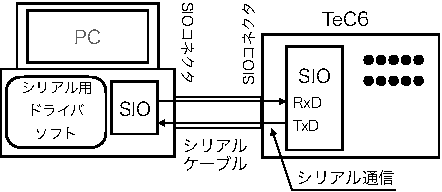
\includegraphics[scale=1.0]{../Keynote/serial5-crop.pdf}}
\end{frame}

%==============================================================================
\begin{frame}
  \frametitle{PCとUSBで接続する}
  PCとUSBケーブルで接続するとシリアル通信が可能になる.
  \begin{itemize}
    \item USBケーブルで電源も供給される
    \item TeCが「USB--シリアル変換LSI(FT232RL)」を内蔵
    \item FT232RLとSIOインタフェース間だけがシリアル通信
    \item FT232RL用ドライバがPC上のソフトにSIO通信機能を提供
    \item FT232RL用ドライバはmacOSに標準で装備されている
    \item TeCのプログラムは昔と同じ方法で通信ができる
  \end{itemize}
  \centerline{\includegraphics[scale=1.0]{../Keynote/serial6-crop.pdf}}
\end{frame}

%==============================================================================
\begin{frame}
  \frametitle{PCとBluetoothで接続する}
  PCとBluetooth(無線)で接続しシリアル通信を行う.
  \begin{itemize}
    \item TeCが「Bluetooth--シリアル変換LSI(RN4020)」を内蔵
    \item RN4020とSIOインタフェース間だけがシリアル通信
    \item Macには専用のアプリ(BlueTerminal)が必要
    \item USB接続とBluetooth接続は同時に使用できる
    \item TeCのプログラムは昔と同じ方法で通信ができる
  \end{itemize}
  \centerline{\includegraphics[scale=1.0]{../Keynote/serial7-crop.pdf}}
\end{frame}

%==============================================================================
\begin{frame}
  \frametitle{シリアル入出力回路の仕組み}
  TeCのSIOインタフェース回路の仕組み
  \begin{itemize}
    \item 受信したシリアルデータはシフトレジスタで8bitまとめる
    \item 8bitまとまったら受信バッファに移し,次の受信に備える
    \item シフトレジスタが空になったら送信バッファからデータが移される
    \item シフトレジスタで1bitずつに分解して出力する
  \end{itemize}
  \centerline{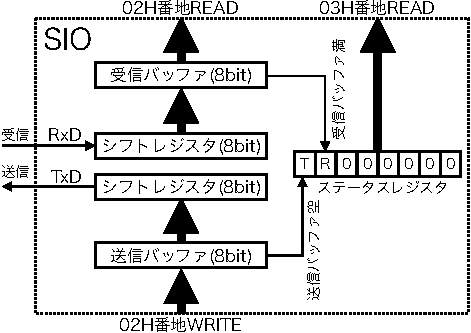
\includegraphics[scale=0.85]{../Keynote/sio-crop.pdf}}
\end{frame}

%==============================================================================
\begin{frame}
  \frametitle{I/Oポート}
  TeCのプログラムがSIOインタフェース回路をアクセスするI/O番地
  \centerline{\begin{tabular}{| c | l | l |}
    \hline
    番地 & read(IN命令) & write(OUT命令) \\\hline
    02H  & 受信バッファ & 送信バッファ   \\\hline
    03H  & ステータス   & コントロール   \\\hline
    \end{tabular}
  }
  \begin{itemize}
    \item 02H番地から受信・送信バッファの読み書きができる
    \item 03H番地で受信・送信バッファの状態を知ることができる
    \item ステータスの意味は次の通り
  \end{itemize}
  \centerline{\includegraphics[scale=1.2]{../chap5/serial3.pdf}}
\end{frame}

%==============================================================================
\begin{frame}
  \frametitle{シリアル出力プログラム}
  SIOへ1文字出力するプログラムの例
  \begin{itemize}
    \item ステータスのTビットが1になるまで待つ
    \item 送信バッファに送信データを書き込む
  \end{itemize}
  \centerline{\includegraphics[scale=0.85]{../Tikz/flow6.pdf}}
\end{frame}

%==============================================================================
\begin{frame}
  \frametitle{シリアル入力プログラム}
  SIOから1文字入力するプログラムの例
  \begin{itemize}
    \item ステータスのRビットが1になるまで待つ
    \item 受信バッファから受信データを読み取る
  \end{itemize}
  \centerline{\includegraphics[scale=0.85]{../Tikz/flow7.pdf}}
\end{frame}

%==============================================================================
\begin{frame}[fragile]
  \frametitle{シリアル通信アプリ}
  Mac側でSIO通信に使用する通信プログラム(screenコマンド)
  \begin{itemize}
    \item SIOから受信したデータを文字コードとみなし表示
    \item 押されたキーに対応する文字コードをSIOへ送信
  \end{itemize}

\begin{framed}{\small
\begin{verbatim}
1. TeCとMacをUSBケーブルで接続する
2. ターミナルで次のように操作する

% screen /dev/cu.usb[TAB][Enter] # TAB, Enter を順に入力する
... 通信画面になる ...
[^A][^¥]y                        # Ctrl-A, Ctrl-¥, y で終了
%
\end{verbatim}
}\end{framed}
\end{frame}

%==============================================================================
\begin{frame}
  \frametitle{まとめ}
  \emph{学んだこと}
  \begin{itemize}
  \item シリアル入出力の仕組み
  \item TeCのシリアル入出力回路の仕組み
  \item シリアル入出力プログラムの作り方
  \item Macの通信プログラム(screen)
  \end{itemize}
  \vfill
  \emph{演習}
  \begin{itemize}
  \item 「例題5-9 `A'〜`Z'の文字を出力」を試しなさい.
  \item 「例題5-10 echo プログラム」を試しなさい.
  \item 受信した文字を「カエサル暗号」にして送り返すプログラムを作りなさい.
  (文字はA-Zの26種類だけ.受信した文字を辞書順で前に3文字シフトする)
  \end{itemize}
  \vfill
\end{frame}

\end{document}
